% Created 2021-08-05 to 17:48
% Intended LaTeX compiler: pdflatex
\documentclass[12pt]{article}

%%%% settings when exporting code %%%% 

\usepackage{listings}
\lstdefinestyle{code-small}{
backgroundcolor=\color{white}, % background color for the code block
basicstyle=\ttfamily\small, % font used to display the code
commentstyle=\color[rgb]{0.5,0,0.5}, % color used to display comments in the code
keywordstyle=\color{black}, % color used to highlight certain words in the code
numberstyle=\ttfamily\tiny\color{gray}, % color used to display the line numbers
rulecolor=\color{black}, % color of the frame
stringstyle=\color[rgb]{0,.5,0},  % color used to display strings in the code
breakatwhitespace=false, % sets if automatic breaks should only happen at whitespace
breaklines=true, % sets automatic line breaking
columns=fullflexible,
frame=single, % adds a frame around the code (non,leftline,topline,bottomline,lines,single,shadowbox)
keepspaces=true, % % keeps spaces in text, useful for keeping indentation of code
literate={~}{$\sim$}{1}, % symbol properly display via latex
numbers=none, % where to put the line-numbers; possible values are (none, left, right)
numbersep=10pt, % how far the line-numbers are from the code
showspaces=false,
showstringspaces=false,
stepnumber=1, % the step between two line-numbers. If it's 1, each line will be numbered
tabsize=1,
xleftmargin=0cm,
emph={anova,apply,class,coef,colnames,colNames,colSums,dim,dcast,for,ggplot,head,if,ifelse,is.na,lapply,list.files,library,logLik,melt,plot,require,rowSums,sapply,setcolorder,setkey,str,summary,tapply},
aboveskip = \medskipamount, % define the space above displayed listings.
belowskip = \medskipamount, % define the space above displayed listings.
lineskip = 0pt} % specifies additional space between lines in listings
\lstset{style=code-small}
%%%% packages %%%%%

\usepackage[utf8]{inputenc}
\usepackage[T1]{fontenc}
\usepackage{lmodern}
\usepackage{textcomp}
\usepackage{color}
\usepackage{graphicx}
\usepackage{grffile}
\usepackage{wrapfig}
\usepackage{rotating}
\usepackage{longtable}
\usepackage{multirow}
\usepackage{multicol}
\usepackage{changes}
\usepackage{pdflscape}
\usepackage{geometry}
\usepackage[normalem]{ulem}
\usepackage{amssymb}
\usepackage{amsmath}
\usepackage{amsfonts}
\usepackage{dsfont}
\usepackage{array}
\usepackage{ifthen}
\usepackage{hyperref}
\usepackage{natbib}
\RequirePackage{setspace} % to modify the space between lines - incompatible with footnote in beamer
\renewcommand{\baselinestretch}{1.1}
\geometry{top=1cm}
\usepackage{titlesec}
\usepackage{etoolbox}

\makeatletter
\patchcmd{\ttlh@hang}{\parindent\z@}{\parindent\z@\leavevmode}{}{}
\patchcmd{\ttlh@hang}{\noindent}{}{}{}
\makeatother
\RequirePackage{colortbl} % arrayrulecolor to mix colors
\definecolor{myorange}{rgb}{1,0.2,0}
\definecolor{mypurple}{rgb}{0.7,0,8}
\definecolor{mycyan}{rgb}{0,0.6,0.6}
\newcommand{\lightblue}{blue!50!white}
\newcommand{\darkblue}{blue!80!black}
\newcommand{\darkgreen}{green!50!black}
\newcommand{\darkred}{red!50!black}
\definecolor{gray}{gray}{0.5}
\hypersetup{
citecolor=[rgb]{0,0.5,0},
urlcolor=[rgb]{0,0,0.5},
linkcolor=[rgb]{0,0,0.5},
}
\newenvironment{note}{\small \color{gray}\fontfamily{lmtt}\selectfont}{\par}
\newenvironment{activity}{\color{orange}\fontfamily{qzc}\selectfont}{\par}
\RequirePackage{pifont}
\RequirePackage{relsize}
\newcommand{\Cross}{{\raisebox{-0.5ex}%
{\relsize{1.5}\ding{56}}}\hspace{1pt} }
\newcommand{\Valid}{{\raisebox{-0.5ex}%
{\relsize{1.5}\ding{52}}}\hspace{1pt} }
\newcommand{\CrossR}{ \textcolor{red}{\Cross} }
\newcommand{\ValidV}{ \textcolor{green}{\Valid} }
\usepackage{stackengine}
\usepackage{scalerel}
\newcommand\Warning[1][3ex]{%
\renewcommand\stacktype{L}%
\scaleto{\stackon[1.3pt]{\color{red}$\triangle$}{\tiny\bfseries !}}{#1}%
\xspace
}
\newcommand\Rlogo{\textbf{\textsf{R}}\xspace} %
\RequirePackage{fancyvrb}
\DefineVerbatimEnvironment{verbatim}{Verbatim}{fontsize=\small,formatcom = {\color[rgb]{0.5,0,0}}}
\RequirePackage{enumitem} % better than enumerate
\RequirePackage{epstopdf} % to be able to convert .eps to .pdf image files
\RequirePackage{capt-of} %
\RequirePackage{caption} % newlines in graphics
\RequirePackage{tikz-cd} % graph
\RequirePackage{booktabs} % for nice lines in table (e.g. toprule, bottomrule, midrule, cmidrule)
\RequirePackage{amsmath}
\RequirePackage{algorithm}
\RequirePackage[noend]{algpseudocode}
\RequirePackage{dsfont}
\RequirePackage{amsmath,stmaryrd,graphicx}
\RequirePackage{prodint} % product integral symbol (\PRODI)
\usepackage{ifthen}
\usepackage{xifthen}
\usepackage{xargs}
\usepackage{xspace}
\newcommand\defOperator[7]{%
\ifthenelse{\isempty{#2}}{
\ifthenelse{\isempty{#1}}{#7{#3}#4}{#7{#3}#4 \left#5 #1 \right#6}
}{
\ifthenelse{\isempty{#1}}{#7{#3}#4_{#2}}{#7{#3}#4_{#1}\left#5 #2 \right#6}
}
}
\newcommand\defUOperator[5]{%
\ifthenelse{\isempty{#1}}{
#5\left#3 #2 \right#4
}{
\ifthenelse{\isempty{#2}}{\underset{#1}{\operatornamewithlimits{#5}}}{
\underset{#1}{\operatornamewithlimits{#5}}\left#3 #2 \right#4}
}
}
\newcommand{\defBoldVar}[2]{
\ifthenelse{\equal{#2}{T}}{\boldsymbol{#1}}{\mathbf{#1}}
}
\newcommandx\Esp[2][1=,2=]{\defOperator{#1}{#2}{E}{}{\lbrack}{\rbrack}{\mathbb}}
\newcommandx\Prob[2][1=,2=]{\defOperator{#1}{#2}{P}{}{\lbrack}{\rbrack}{\mathbb}}
\newcommandx\Qrob[2][1=,2=]{\defOperator{#1}{#2}{Q}{}{\lbrack}{\rbrack}{\mathbb}}
\newcommandx\Var[2][1=,2=]{\defOperator{#1}{#2}{V}{ar}{\lbrack}{\rbrack}{\mathbb}}
\newcommandx\Cov[2][1=,2=]{\defOperator{#1}{#2}{C}{ov}{\lbrack}{\rbrack}{\mathbb}}
\newcommandx\Binom[2][1=,2=]{\defOperator{#1}{#2}{B}{}{(}{)}{\mathcal}}
\newcommandx\Gaus[2][1=,2=]{\defOperator{#1}{#2}{N}{}{(}{)}{\mathcal}}
\newcommandx\Wishart[2][1=,2=]{\defOperator{#1}{#2}{W}{ishart}{(}{)}{\mathcal}}
\newcommandx\Likelihood[2][1=,2=]{\defOperator{#1}{#2}{L}{}{(}{)}{\mathcal}}
\newcommandx\logLikelihood[2][1=,2=]{\defOperator{#1}{#2}{\ell}{}{(}{)}{}}
\newcommandx\Information[2][1=,2=]{\defOperator{#1}{#2}{I}{}{(}{)}{\mathcal}}
\newcommandx\Score[2][1=,2=]{\defOperator{#1}{#2}{S}{}{(}{)}{\mathcal}}
\newcommandx\Vois[2][1=,2=]{\defOperator{#1}{#2}{V}{}{(}{)}{\mathcal}}
\newcommandx\IF[2][1=,2=]{\defOperator{#1}{#2}{IF}{}{(}{)}{\mathcal}}
\newcommandx\Ind[1][1=]{\defOperator{}{#1}{1}{}{(}{)}{\mathds}}
\newcommandx\Max[2][1=,2=]{\defUOperator{#1}{#2}{(}{)}{min}}
\newcommandx\Min[2][1=,2=]{\defUOperator{#1}{#2}{(}{)}{max}}
\newcommandx\argMax[2][1=,2=]{\defUOperator{#1}{#2}{(}{)}{argmax}}
\newcommandx\argMin[2][1=,2=]{\defUOperator{#1}{#2}{(}{)}{argmin}}
\newcommandx\cvD[2][1=D,2=n \rightarrow \infty]{\xrightarrow[#2]{#1}}
\newcommandx\Hypothesis[2][1=,2=]{
\ifthenelse{\isempty{#1}}{
\mathcal{H}
}{
\ifthenelse{\isempty{#2}}{
\mathcal{H}_{#1}
}{
\mathcal{H}^{(#2)}_{#1}
}
}
}
\newcommandx\dpartial[4][1=,2=,3=,4=\partial]{
\ifthenelse{\isempty{#3}}{
\frac{#4 #1}{#4 #2}
}{
\left.\frac{#4 #1}{#4 #2}\right\rvert_{#3}
}
}
\newcommandx\dTpartial[3][1=,2=,3=]{\dpartial[#1][#2][#3][d]}
\newcommandx\ddpartial[3][1=,2=,3=]{
\ifthenelse{\isempty{#3}}{
\frac{\partial^{2} #1}{\partial #2^2}
}{
\frac{\partial^2 #1}{\partial #2\partial #3}
}
}
\newcommand\Real{\mathbb{R}}
\newcommand\Rational{\mathbb{Q}}
\newcommand\Natural{\mathbb{N}}
\newcommand\trans[1]{{#1}^\intercal}%\newcommand\trans[1]{{\vphantom{#1}}^\top{#1}}
\newcommand{\independent}{\mathrel{\text{\scalebox{1.5}{$\perp\mkern-10mu\perp$}}}}
\newcommand\half{\frac{1}{2}}
\newcommand\normMax[1]{\left|\left|#1\right|\right|_{max}}
\newcommand\normTwo[1]{\left|\left|#1\right|\right|_{2}}
\newcommand\Veta{\boldsymbol{\eta}}
\newcommand\VX{\mathbf{X}}
\newcommand\sample{\chi}
\newcommand\Hspace{\mathcal{H}}
\newcommand\Tspace{\mathcal{T}}
\author{Brice Ozenne}
\date{\today}
\title{Inverse probability of censoring weighting (IPCW) for linear regression}
\hypersetup{
 colorlinks=true,
 pdfauthor={Brice Ozenne},
 pdftitle={Inverse probability of censoring weighting (IPCW) for linear regression},
 pdfkeywords={},
 pdfsubject={},
 pdfcreator={Emacs 27.1 (Org mode 9.4.5)},
 pdflang={English}
 }
\begin{document}

\maketitle

\section{Principle}
\label{sec:orgfa612b9}

Inverse probability of censoring weighting (IPCW) is a method able to
handle informative drop-out. Intuitively, in presence of informative
drop-out a complete case analysis is a biased approach as individuals
with complete data are not representative of the population. However
with an appropriate re-weighting of the individuals with complete
data, we can "re-balance" our sample and make it representative of the
population. To do so, we divide the population into sub-populations
and attribute weights to individuals who did not drop-out inversely
proportional to the frequency of the drop-out in the
sub-population. Thanks to the weights, individuals who did not
drop-out "represent" the individuals who dropped-out. Thus, overall,
the weighted sample is representative of the population.

\section{Continuous outcome}
\label{sec:orgde7e51b}

\subsection{Illustrative example}
\label{sec:org04d3e09}

Consider a study were we follow depressed individual over time. They
have a baseline measurement, then are given a treatment, and then have
a follow-up measurement. We would like to assess the treatment effect
in term of depression score \footnote{:To simplfy, there is no control
group - we assume that without treatment the depression score would be
constant.}. The population of interest contain severely and moderately
depressed individuals; the treatment may work differently in each
sub-population. Unfortunately, some study participants dropped-out and
it seems that they are more likely to drop-out when they are severaey
depressed.

\clearpage

We can simulate such a dataset using the following function:
\lstset{language=r,label= ,caption= ,captionpos=b,numbers=none}
\begin{lstlisting}
simTrial <- function(n, rho, dmu, pC){
  require(mvtnorm)
  require(data.table)
  ## simulate data
  Sigma <- 10^2*matrix(c(1,rho,rho,1),2,2)
  ## gather into dataset
  M.Ym <- rmvnorm(n, mean = c(50, 50-dmu[1]), sigma = Sigma)
  M.Ys <- rmvnorm(n, mean = c(75, 75-dmu[2]), sigma = Sigma)
  dtL <- rbind(
    data.table(id = 1:n, mdd = "moderate", time = "T1", Y = M.Ym[,1]),
    data.table(id = 1:n, mdd = "moderate", time = "T2", Y = M.Ym[,2]),
    data.table(id = n+(1:n), mdd = "severe", time = "T1", Y = M.Ys[,1]),
    data.table(id = n+(1:n), mdd = "severe", time = "T2", Y = M.Ys[,2])
  )
  dtL$probaDO <- 0
  dtL[time=="T2", probaDO := ifelse(.SD$mdd=="moderate",pC[1],pC[2])]
  dtL[,dropout := rbinom(.N,prob=probaDO,size=1)]
  dtL[,Yobs:=Y]
  dtL[dropout==1,Yobs:=NA]
  dtL$probaDO <- NULL
  return(dtL)
}
set.seed(11)
dtL <- simTrial(n = 1000, rho = 0.8, dmu = c(25,50), pC = c(0.2,0.7))
print(dtL)
\end{lstlisting}

\begin{verbatim}
        id      mdd time        Y dropout     Yobs
   1:    1 moderate   T1 44.83259       0 44.83259
   2:    2 moderate   T1 30.34157       0 30.34157
   3:    3 moderate   T1 56.36308       0 56.36308
   4:    4 moderate   T1 64.63341       0 64.63341
   5:    5 moderate   T1 45.10048       0 45.10048
  ---                                             
3996: 1996   severe   T2 30.59793       1       NA
3997: 1997   severe   T2 18.97725       1       NA
3998: 1998   severe   T2 29.80266       1       NA
3999: 1999   severe   T2 30.26518       0 30.26518
4000: 2000   severe   T2 39.15797       0 39.15797
\end{verbatim}

Here we have simulated a two sub-populations of 1000, with a
correlation of 0.5 between baseline and follow-up . The treatment
effect is twice bigger for the severely depressed population but
individuals from this population are also much more likely to
drop-out. Overall the expected treatment effect is:
\lstset{language=r,label= ,caption= ,captionpos=b,numbers=none}
\begin{lstlisting}
(-25-50)/2
\end{lstlisting}

\begin{verbatim}
[1] -37.5
\end{verbatim}


\bigskip

Without drop-out, we could use a simple linear model to carry-out the analysis:
\lstset{language=r,label= ,caption= ,captionpos=b,numbers=none}
\begin{lstlisting}
dtW.oracle <- dcast(dtL, formula = id ~ time, value.var = "Y")
dtW.oracle$diff <- dtW.oracle$T2-dtW.oracle$T1
e.oracle <- lm(diff~1, data = dtW.oracle)
summary(e.oracle)$coef
\end{lstlisting}

\begin{verbatim}
             Estimate Std. Error   t value Pr(>|t|)
(Intercept) -37.35098  0.3141814 -118.8835        0
\end{verbatim}

leading to an estimate quite close to the true value.

\bigskip

With drop-out, a complete case analysis would lead to a biased
estimator. In this example, we can "see" that the estimated value is
far away from the true one (even when accouting for the uncertainty):
\lstset{language=r,label= ,caption= ,captionpos=b,numbers=none}
\begin{lstlisting}
dtW <- dcast(dtL, formula = id + mdd ~ time, value.var = "Yobs")
dtW$diff <- dtW$T2-dtW$T1
dtW.CC <- dtW[!is.na(diff)]
e.CC <- lm(diff~1, data = dtW.CC)
summary(e.CC)$coef
\end{lstlisting}

\begin{verbatim}
             Estimate Std. Error   t value Pr(>|t|)
(Intercept) -31.42356  0.3909029 -80.38713        0
\end{verbatim}


An alternative approach would be to use a linear mixed model
(i.e. full information):
\lstset{language=r,label= ,caption= ,captionpos=b,numbers=none}
\begin{lstlisting}
require(nlme)
e.FI <- lme(Yobs~time, random = ~1|id, data = dtL, na.action = na.omit)
summary(e.FI)$tTable
\end{lstlisting}

\begin{verbatim}
                Value Std.Error   DF   t-value p-value
(Intercept)  62.59128 0.3239587 1999 193.20760       0
timeT2      -33.76472 0.3855964 1068 -87.56494       0
\end{verbatim}

which is better than the complete case analysis still biased when the
drop-out mechanism depends on variables other than the baseline value.

\clearpage

 A better approach is to use IPCW. First we model the probability of
not dropping out at follow-up:
\lstset{language=r,label= ,caption= ,captionpos=b,numbers=none}
\begin{lstlisting}
dtW$observed <- !is.na(dtW$T2)
e.glmW.oracle <- glm(observed ~ mdd, data = dtW,
		     family = binomial(link = "logit"))
\end{lstlisting}

and then compute the weights for observations with full data:
\lstset{language=r,label= ,caption= ,captionpos=b,numbers=none}
\begin{lstlisting}
dtW$weight.oracle <- 1/predict(e.glmW.oracle, newdata = dtW,type = "response")
dtW[observed == TRUE, sum(weight.oracle)]
\end{lstlisting}

\begin{verbatim}
[1] 2000
\end{verbatim}


Note that the weights sum to the total sample size. We then perform
the complete case analysis with these weights:
\lstset{language=r,label= ,caption= ,captionpos=b,numbers=none}
\begin{lstlisting}
dtW.CC <- dtW[!is.na(diff)]
e.IPCWoracle <- lm(diff~1, data = dtW.CC, weights = dtW.CC$weight.oracle)
summary(e.IPCWoracle)$coef
\end{lstlisting}

\begin{verbatim}
             Estimate Std. Error  t value Pr(>|t|)
(Intercept) -36.89889  0.4251421 -86.7919        0
\end{verbatim}


which gives a result much closer to the true value. A more feasible
IPCW would use the baseline score to define the weights:
\lstset{language=r,label= ,caption= ,captionpos=b,numbers=none}
\begin{lstlisting}
e.glmW <- glm(observed ~ T1, data = dtW,
	      family = binomial(link = "logit"))
dtW$weight <- 1/predict(e.glmW, newdata = dtW, type = "response")
dtW[observed == TRUE, sum(weight)]
\end{lstlisting}

\begin{verbatim}
[1] 2015.739
\end{verbatim}


We then perform the complete case analysis with these new weights:
\lstset{language=r,label= ,caption= ,captionpos=b,numbers=none}
\begin{lstlisting}
dtW.CC <- dtW[!is.na(diff)]
e.IPCW <- lm(diff~1, data = dtW.CC, weights = dtW.CC$weight)
summary(e.IPCW)$coef
\end{lstlisting}

\begin{verbatim}
             Estimate Std. Error   t value Pr(>|t|)
(Intercept) -35.47206   0.423423 -83.77453        0
\end{verbatim}


\clearpage

\subsection{Simulation study}
\label{sec:org873771e}

The quality of the previous estimators is compared using a simulation
study. The results are summarized by \autoref{fig:simulationGaussian}.

\begin{figure}[!h]
\centering
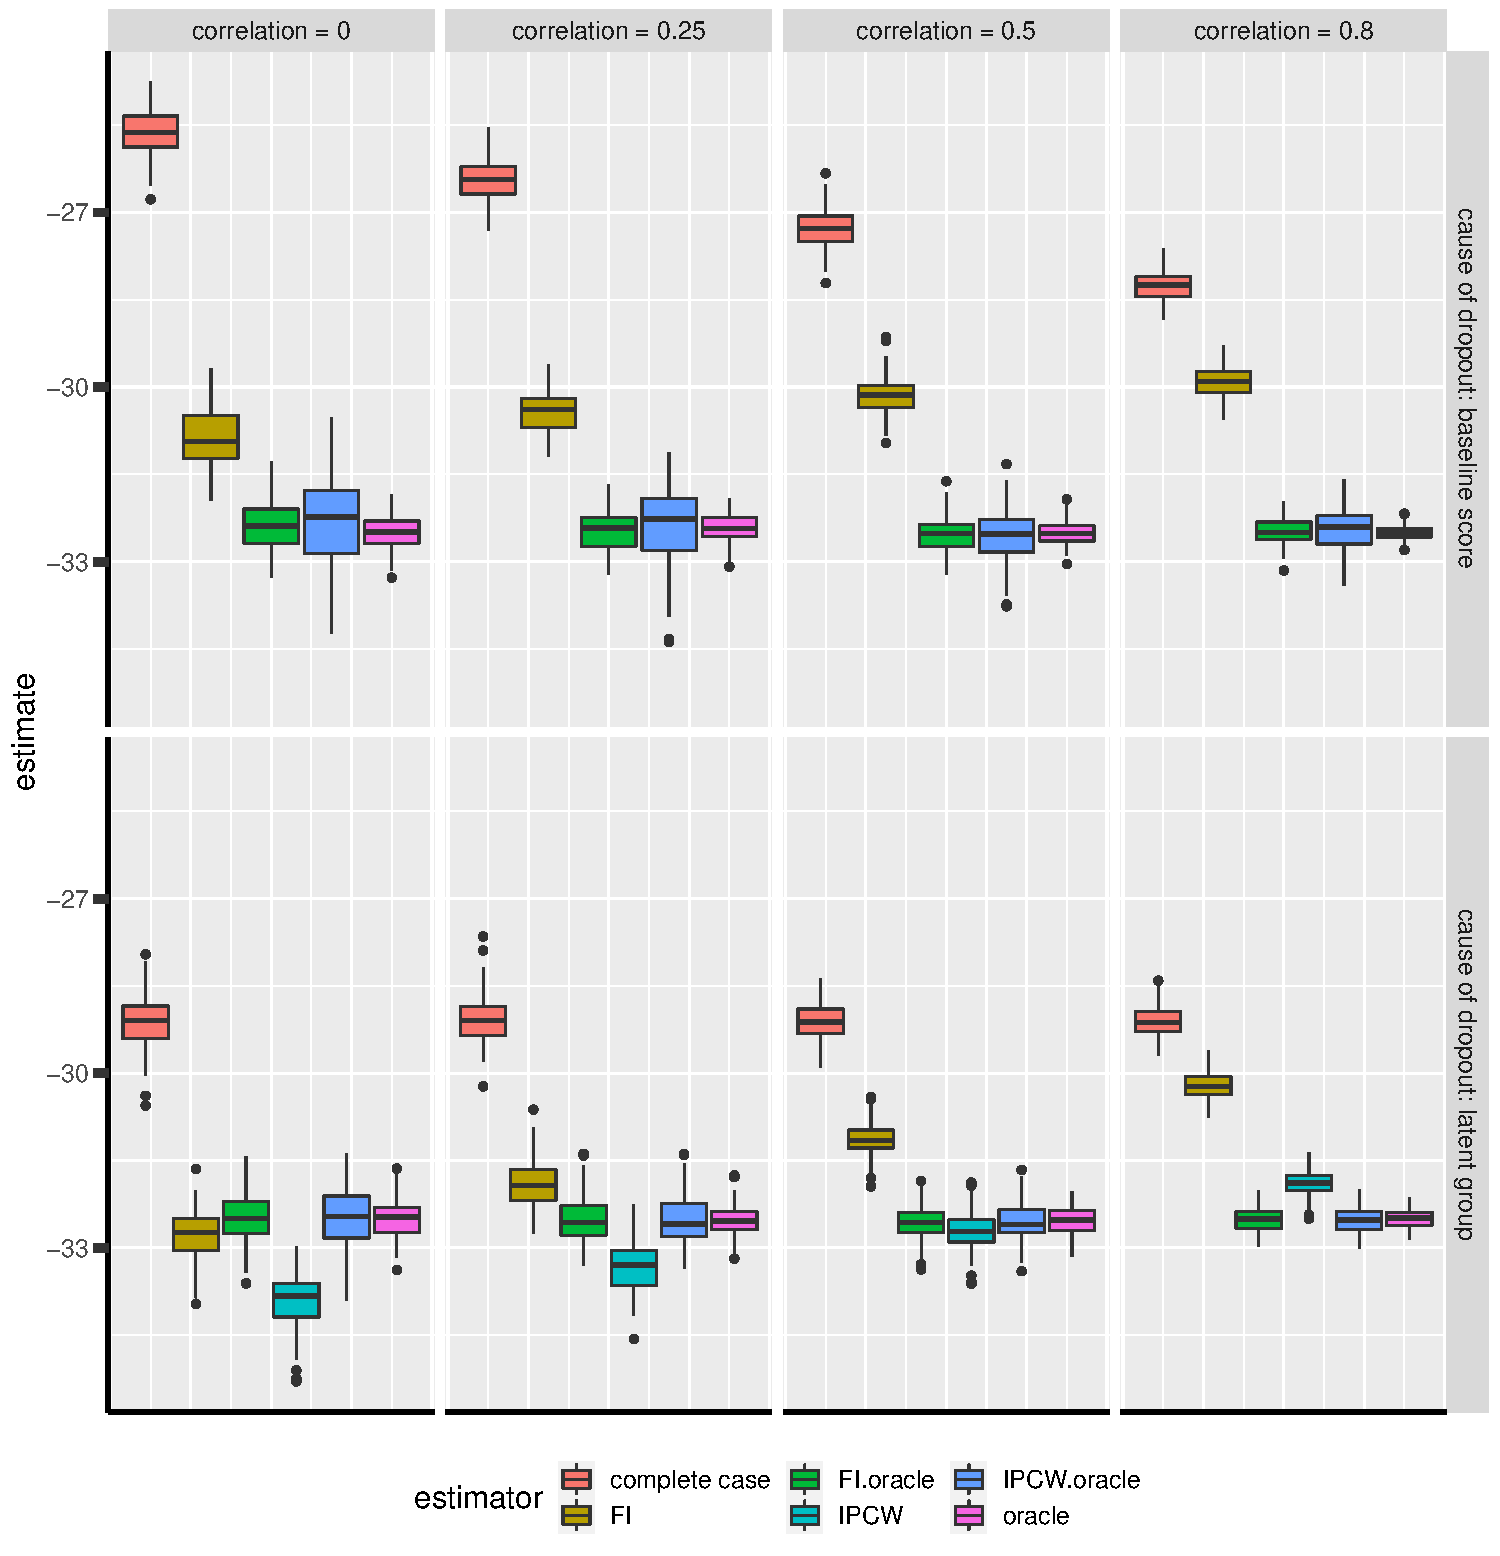
\includegraphics[width=\textwidth]{./figures/simStudy-bias.pdf}
\caption{\label{fig:simulationGaussian}Comparison between the empirical distributions of the estimators (Gaussian case) for a sample size of 1000 using 100 datasets.}
\end{figure}

\bigskip

\section{Binary outcome}
\label{sec:org0e97245}

\subsection{Illustrative example}
\label{sec:org6e6b4dd}
A somehow similar approach can be used for binary endpoints. Consider
now a study comparing the survival probability at 1 year of patients
treated with a new drug vs. standard care. The population is composed
of two types of patients, say some with hypertension and some
without. Survival as well as the treatment effect may differ depending
of the hypertension status. Hypertension may also affect the drop-out
probability.

\clearpage

We can simulate such a dataset using the following function:
\lstset{language=r,label= ,caption= ,captionpos=b,numbers=none}
\begin{lstlisting}
simTrial <- function(n, dmu, dpC){
  require(BuyseTest)
  require(data.table)
  ## simulate data
  dt1  <- simBuyseTest(n.T = n, n.C = n, 
		       argsBin = NULL, argsCont = NULL, 
		       argsTTE = list(scale.T = 1+dmu[1],
				      scale.C = 1,
				      scale.Censoring.T = 1+dpC[1],
				      scale.Censoring.C = 1),
		       latent = TRUE)
  dt2  <- simBuyseTest(n.T = n, n.C = n, 
		       argsBin = NULL, argsCont = NULL, 
		       argsTTE = list(scale.T = 2+dmu[2],
				      scale.C = 2,
				      scale.Censoring.T = 2+dpC[2],
				      scale.Censoring.C = 2),
		       latent = TRUE)
  ## gather into dataset
  dt <- rbind(
    cbind(id = 1:NROW(dt1), group = "G1", dt1),
    cbind(id = NROW(dt1) + 1:NROW(dt2), group = "G2", dt2)
  )
  return(dt)
}
set.seed(11)
tau <- 1

dt <- simTrial(n = 10000, dmu = c(0,1), dpC = c(0,1))
dt$responseUncensored <- dt$eventtimeUncensored<=tau
dt$response <- ifelse((dt$status==1)+(dt$eventtime>tau),dt$eventtime<=tau,NA)
dt$observed <- ifelse((dt$status==1)+(dt$eventtime>tau),1,0)
print(dt)
\end{lstlisting}

\begin{verbatim}
          id group treatment eventtimeUncensored eventtimeCensoring  eventtime
    1:     1    G1         C          1.63238841         1.74283865 1.63238841
    2:     2    G1         C          0.08938341         1.10407172 0.08938341
    3:     3    G1         C          1.54194414         1.11212966 1.11212966
    4:     4    G1         C          1.04592013         1.00584279 1.00584279
    5:     5    G1         C          0.55276522         0.04955419 0.04955419
   ---                                                                        
39996: 39996    G2         T          4.08919433         1.23091105 1.23091105
39997: 39997    G2         T          3.59736307         8.14939225 3.59736307
39998: 39998    G2         T          7.21110232         3.04114191 3.04114191
39999: 39999    G2         T          0.06096057         0.42120185 0.06096057
40000: 40000    G2         T          6.89615584         2.22637070 2.22637070
       status responseUncensored response observed
    1:      1              FALSE    FALSE        1
    2:      1               TRUE     TRUE        1
    3:      0              FALSE    FALSE        1
    4:      0              FALSE    FALSE        1
    5:      0               TRUE       NA        0
   ---                                            
39996:      0              FALSE    FALSE        1
39997:      1              FALSE    FALSE        1
39998:      0              FALSE    FALSE        1
39999:      1               TRUE     TRUE        1
40000:      0              FALSE    FALSE        1
\end{verbatim}

In absence of drop-out, we can compare the survival
probabilities at 1 year using a logistic regression:
\lstset{language=r,label= ,caption= ,captionpos=b,numbers=none}
\begin{lstlisting}
e.oracle <- glm(responseUncensored ~ treatment,
		data = dt, family = binomial(link="logit"))
summary(e.oracle)$coef
\end{lstlisting}

\begin{verbatim}
               Estimate Std. Error   z value     Pr(>|z|)
(Intercept)  0.07022885 0.01415085   4.96287 6.945906e-07
treatmentT  -0.23721580 0.02004104 -11.83650 2.527721e-32
\end{verbatim}


In presence of (differential) drop-out, a complete case analysis
(i.e. restricting the analysis to the patients where the survival
status at 1 year is known) would be biased:
\lstset{language=r,label= ,caption= ,captionpos=b,numbers=none}
\begin{lstlisting}
dt.cc <- dt[dt$observed==1]
e.cc <- glm(response ~ treatment,
	    data = dt.cc, family = binomial(link="logit"))
summary(e.cc)$coef
\end{lstlisting}

\begin{verbatim}
              Estimate Std. Error   z value      Pr(>|z|)
(Intercept)  0.4023018 0.01814959  22.16589 7.330653e-109
treatmentT  -0.3656280 0.02510139 -14.56605  4.618541e-48
\end{verbatim}


A first idea would be to re-use the IPCW approach, first fitting a
logistic model for the probability of being observed at 1-year and
then computing the weights:
\lstset{language=r,label= ,caption= ,captionpos=b,numbers=none}
\begin{lstlisting}
e.IPCmodel <- glm(observed ~ group*treatment, data = dt, family = binomial(link="logit"))
dt$IPCweights <- 1/predict(e.IPCmodel, newdata = dt, type = "response")
sum(dt$IPCweights)
\end{lstlisting}

\begin{verbatim}
[1] 62570.28
\end{verbatim}


The subsequent estimator will not be correct: 
\lstset{language=r,label= ,caption= ,captionpos=b,numbers=none}
\begin{lstlisting}
dt.cc <- dt[dt$observed==1]
e.IPCWcc <- glm(response ~ treatment, data = dt.cc,
		family = binomial(link="logit"), weights = dt.cc$IPCweights)
summary(e.IPCWcc)$coef
\end{lstlisting}

\begin{verbatim}
Advarselsbesked:
I eval(family$initialize) : non-integer #successes in a binomial glm!
              Estimate Std. Error   z value      Pr(>|z|)
(Intercept)  0.4593548 0.01451679  31.64300 9.465106e-220
treatmentT  -0.2997806 0.02029810 -14.76889  2.324953e-49
\end{verbatim}


as we disregarded the duration of observation among the censored
individuals. Intuitively, individuals censored early are more at risk
of dying and therefore should "transfer" more weight than those
censored late, e.g. just before 1 year, who don't really need to
transfer weights. This can be perform using a survival model (here a
Cox model) and using as weights the inverse of the probability of not
being censored at the earliest between when the event occured and 1
year:
\lstset{language=r,label= ,caption= ,captionpos=b,numbers=none}
\begin{lstlisting}
library(survival)
library(riskRegression)
e.IPCmodel2 <- coxph(Surv(eventtime,status==0) ~ group*treatment,
		     data = dt, x = TRUE, y = TRUE)
iPred <- predictCox(e.IPCmodel2, newdata = dt,
		    time = pmin(dt$eventtime,tau)-(1e-12), diag = TRUE)$survival
dt$IPCweights2 <- dt$observed/iPred
sum(dt$IPCweights2)
\end{lstlisting}

\begin{verbatim}
[1] 40028.88
\end{verbatim}


We can then use the weights in a logistic model:
\lstset{language=r,label= ,caption= ,captionpos=b,numbers=none}
\begin{lstlisting}
dt.cc <- dt[dt$observed==1]
e.IPCWcc <- glm(response ~ treatment, data = dt.cc, family = binomial(link="logit"), weights = dt.cc$IPCweights2)
summary(e.IPCWcc)$coef
\end{lstlisting}

\begin{verbatim}
Advarselsbesked:
I eval(family$initialize) : non-integer #successes in a binomial glm!
               Estimate Std. Error    z value     Pr(>|z|)
(Intercept)  0.06439848 0.01414818   4.551716 5.321009e-06
treatmentT  -0.23858152 0.02003591 -11.907693 1.079216e-32
\end{verbatim}


which is very close to the true value. Note that this estimator is
implemented in the riskRegression package:
\lstset{language=r,label= ,caption= ,captionpos=b,numbers=none}
\begin{lstlisting}
e.wglm <- wglm(regressor.event = ~treatment,
	       formula.censor = Surv(eventtime,status==0)~group*treatment,
	       times = 1,
	       data = dt[,.(eventtime,status,group,treatment)])
summary(e.wglm)
\end{lstlisting}

\begin{verbatim}
     IPCW logistic regression : 
----------------------------------------------------------------------------------
  - time: 1
glm(XX_status.1_XX ~ treatment, family = binomial(link = "logit"), 
    weights = "XX_IPCW.1_XX")

               Estimate Std. Error   z value     Pr(>|z|)
(Intercept)  0.06439847 0.01931759  3.333670 0.0008570818
treatmentT  -0.23858152 0.02652596 -8.994264 0.0000000000
----------------------------------------------------------------------------------
\end{verbatim}

Another, similar, weighted estimator is implemented in the mets package:
\lstset{language=r,label= ,caption= ,captionpos=b,numbers=none}
\begin{lstlisting}
e.mets <- binreg(formula = Event(eventtime,status) ~ treatment,
		 cens.model = ~group*treatment,
		 time = 1, data = dt, cens.code = 0, cause = 1)
e.mets
\end{lstlisting}

\begin{verbatim}

     n events
 40000  14351

 40000 clusters
log-coeffients:
             Estimate   Std.Err      2.5%     97.5% P-value
(Intercept)  0.064776  0.019716  0.026134  0.103418   0.001
treatmentT  -0.236638  0.027400 -0.290341 -0.182936   0.000

exp(coeffients):
              Estimate  Std.Err     2.5%    97.5% P-value
[(Intercept)] 1.066920 0.021035 1.025692 1.108148  0.0015
[treatmentT]  0.789277 0.021626 0.746890 0.831663  0.0000
\end{verbatim}


\subsection{Simulation study}
\label{sec:org18ddb1f}

The quality of the previous estimators is compared using a simulation
study. The results are summarized by \autoref{fig:simulationBinary} and \autoref{fig:simulationBinarySD} 
\begin{figure}[!h]
\centering
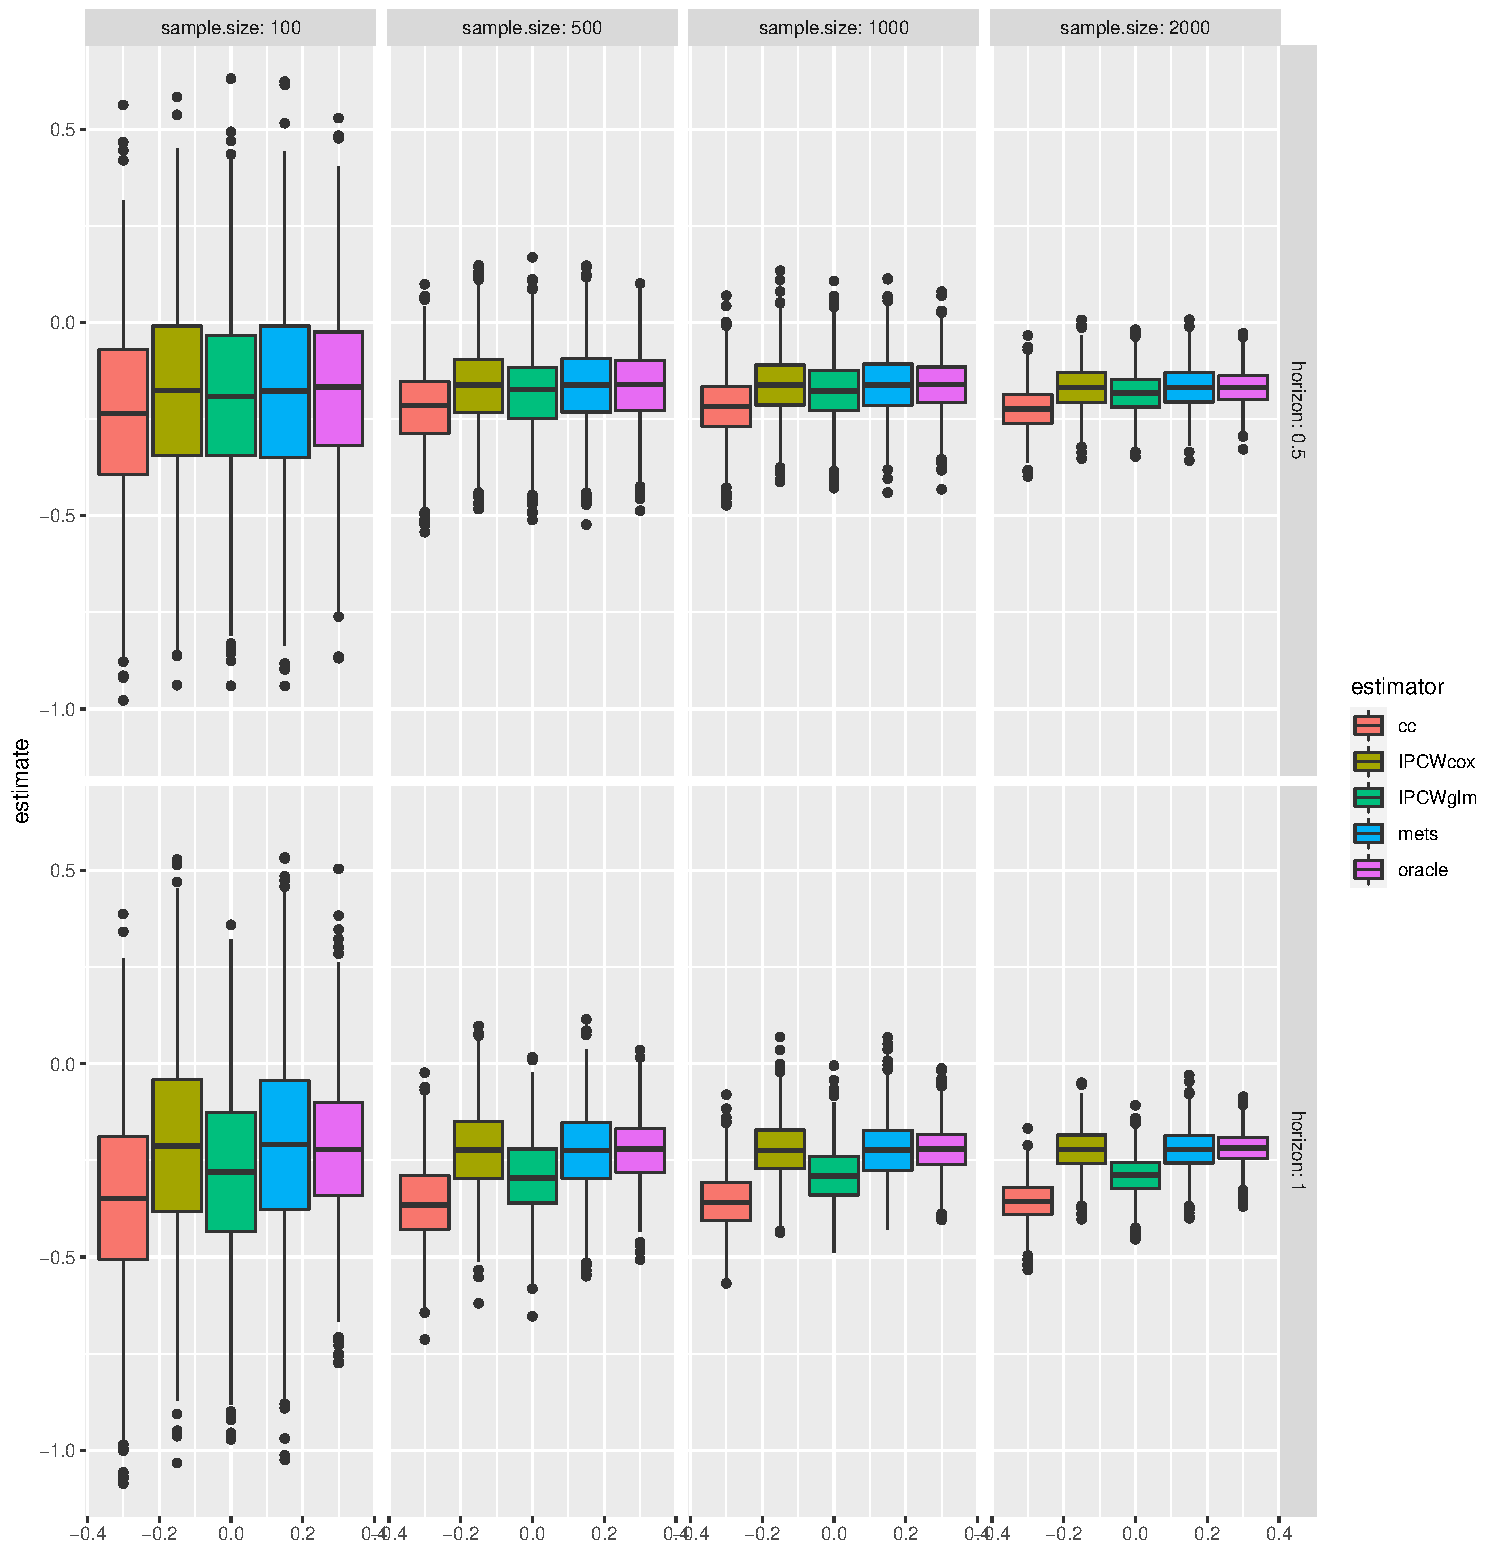
\includegraphics[width=\textwidth]{./figures/simStudy-bin-bias.pdf}
\caption{\label{fig:simulationBinary}Comparison between the empirical distributions of the estimators (binary case) across sample size. Based on 1000 replicates.}
\end{figure}

\begin{figure}[!h]
\centering
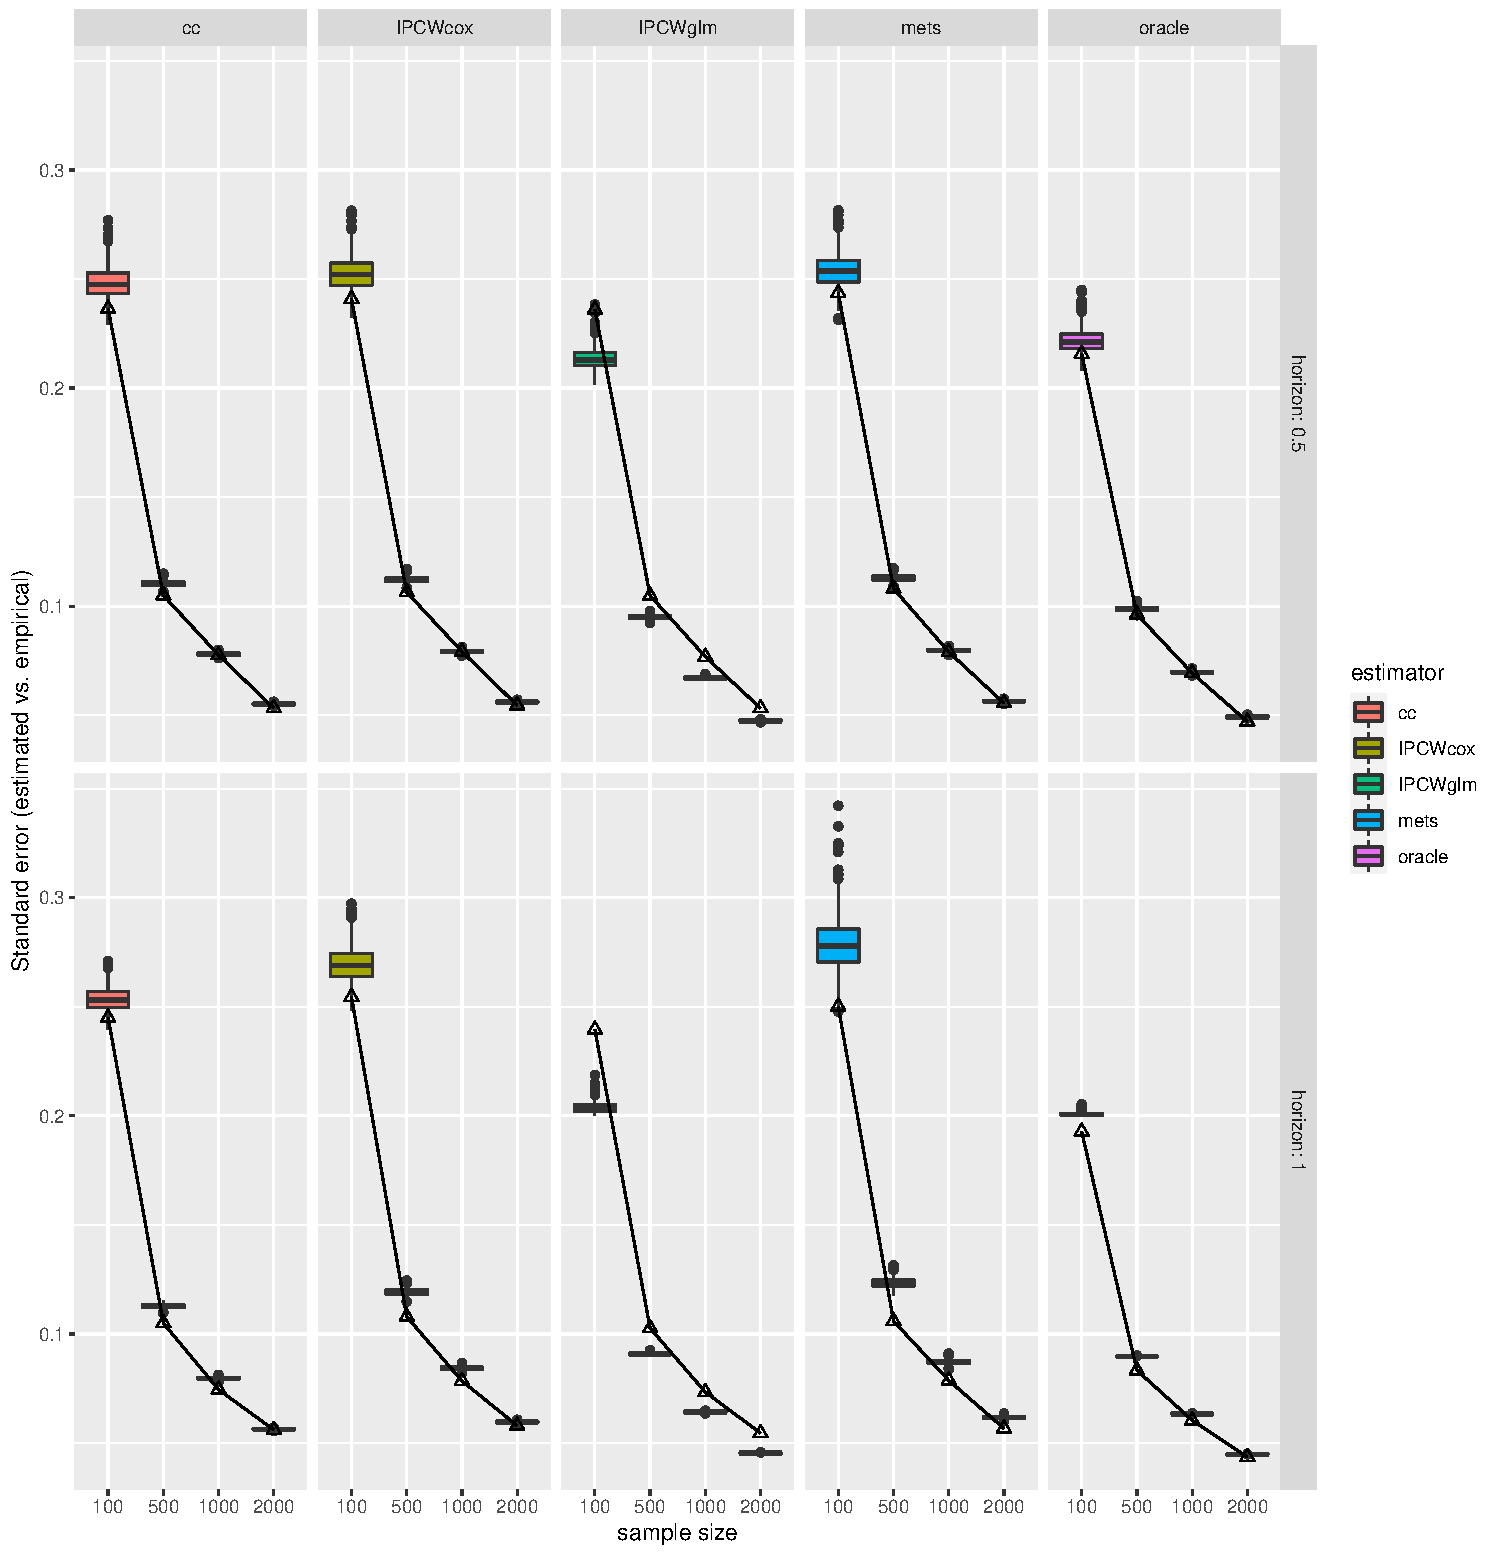
\includegraphics[width=\textwidth]{./figures/simStudy-bin-sd.pdf}
\caption{\label{fig:simulationBinarySD}Comparison between the modeled standard errors of the estimates (boxplot) and the empirical ones (triangles linked by a line) across sample size. Based on 1000 replicates.}
\end{figure}
\end{document}